%!TEX root = paper.tex
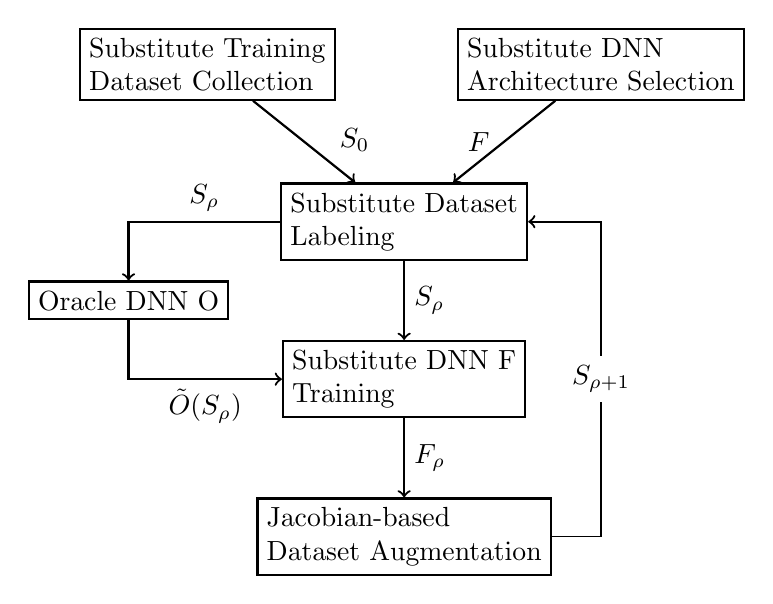
\begin{tikzpicture}[node distance = 2cm, auto]
    \node [rectangle, thick, draw, align=left] (init) at (1,10) {Substitute Training \\ Dataset Collection};
    \node [rectangle, thick, draw, align=left] (selection) at (6,10) {Substitute DNN \\ Architecture Selection};
    \node [rectangle, thick, draw, align=left] (labeling) at (3.5,8) {Substitute Dataset \\ Labeling};
    \node [rectangle, thick, draw, align=left] (training) at (3.5,6) {Substitute DNN F \\ Training};
    \node [rectangle, thick, draw, align=left] (augmentation) at (3.5,4) {Jacobian-based \\ Dataset Augmentation};
    \node [rectangle, thick, draw, align=left] (oracle) at (0,7) {Oracle DNN O};
    \node (helper) at (6,6) {$S_{\rho+1}$};

    \draw[->, thick] (init) -- (labeling) node [near end] {$S_0$};
    \draw[->, thick] (selection) -- (labeling) node [above,near end] {$F$};
    \draw[->, thick] (labeling) -- (training) node [midway] {$S_\rho$};
    \draw[->, thick] (training) -- (augmentation) node [midway] {$F_\rho$};
    \draw[->, thick] (labeling) -| (oracle) node [near start, above] {$S_\rho$};
    \draw[->, thick] (oracle) |- (training) node [near end, below] {$\tilde{O}(S_\rho)$};
    \draw (augmentation) -|  (helper);
    \draw[->, thick] (helper) |- (labeling);
\end{tikzpicture}